\subchapter{Configuring the pin muxing}
{Objective: learn how to declare and use a muxing state.}

\section{Goals}

As part of the previous lab, we enabled an I2C controller and described
a device plugged on the bus. In this lab we will cover how to ensure a
proper communication between the two and be able to declare and use
pinctrl settings.

\section{Setup}

Continue using the \code{beagleplay-custom} branch in the
\code{~/__SESSION_NAME__-labs/src/linux} directory.

\section{Probing the different busses}

The Beagle Play device tree already correctly configures the pinmuxing state
for the I2C3 bus. Before proceeding with this lab, we ask you to delete this
pinmuxing configuration by adding two lines in your custom device tree:

\begin{verbatim}
 &main_i2c3 {
        status = "okay";
+       /delete-property/ pinctrl-0;
+       /delete-property/ pinctrl-names;
\end{verbatim}

Reboot your board with these changes.

Now, let's use \code{i2cdetect}'s capability to probe a bus for
devices. The I2C bus has no real discovery capability, but yet, the tool
exploits a feature of the specification: when the master talks to a
device, it starts by sending the target address on the bus and expects
it to be acked by the relevant device. Iterating through all the
possible addresses without sending anything after the address byte,
looking for the presence of an Ack is what uses the tool to probe the
devices. That is also why we get a warning when using it.

Let's start by probing the bus associated to \code{i2c-0}:

\begin{bashinput}
# i2cdetect -r 0
i2cdetect: WARNING! This program can confuse your I2C bus
Continue? [y/N] y
     0  1  2  3  4  5  6  7  8  9  a  b  c  d  e  f
00:          -- -- -- -- -- -- -- -- -- -- -- -- -- 
10: -- -- -- -- -- -- -- -- -- -- -- -- -- -- -- -- 
20: -- -- -- -- -- -- -- -- -- -- -- -- -- -- -- -- 
30: UU -- -- -- -- -- -- -- -- -- -- -- -- -- -- -- 
40: -- -- -- -- -- -- -- -- -- -- -- -- -- -- -- -- 
50: 50 -- -- -- -- -- -- -- -- -- -- -- -- -- -- -- 
60: -- -- -- -- -- -- -- -- 68 -- -- -- -- -- -- -- 
70: -- -- -- -- -- -- -- -- 
\end{bashinput}

We can see three devices on this internal bus:
\begin{itemize}
\item One at address \code{0x30}, indicated by \code{UU},
      which means that there is a kernel driver actively
      driving this device.
\item Two other devices at addresses \code{0x50} and \code{0x68}.
      We just know that they are currently not bound to a kernel driver.
\end{itemize}

Now try to probe I2C3 with \code{i2cdetect -r 3}.

You will see that the command will fail to connect to
the bus. That's because the corresponding signals are
not exposed yet to the outside connectors through pin muxing.

\section{Find pin muxing configuration information for i2c3}

As you found in the previous lab, we now managed to have our nunchuk
device enumerated on the \code{i2c3} bus.

However, to access the bus data and clock signals, we need to configure
the pin muxing of the SoC.

If you open the Beagle Play hardware schematics and go to sheet 13,
you'll see that the \code{I2C3_SCL} and \code{I2C3_SDA} signals are routed to pins
A15 and B15 on the AM625 SoC.

Now open the AM625 datasheet (not the reference manual!) and go to
table 6.1 in the "Pin Attributes" section. Search for pins A15 and
B15 in this table, using the first column, not the second one.

Once you've found pins A15 and B15, you'll see that mux mode number 2
corresponds to the \code{I2C3_SCL} and \code{ISC3_SDA} signals.

In the third column, you'll find the addresses of the pad configuration
registers for these pins. Register 0x000F41D0 configures A15 and register
0x000F41D4 configures B15.


We now know which registers we can write to to enable \code{i2c3}
signals.

\section{Multiplexing the I2C controller outputs correctly}

Now that we know the register offsets, let's try to understand
how they are used in existing code. Open the original device tree
for the Beagle Play board and go to the \code{main_i2c3} node.
You'll see a handle to a pinctrl node: \code{mikrobus_i2c_pins_default}.
Look for this pinctrl node; you'll see the following description:

\begin{verbatim}
mikrobus_i2c_pins_default: mikrobus-i2c-default-pins {
                pinctrl-single,pins = < 
                        AM62X_IOPAD(0x01d0, PIN_INPUT_PULLUP, 2) /* (A15) UART0_CTSn.I2C3_SCL */
                        AM62X_IOPAD(0x01d4, PIN_INPUT_PULLUP, 2) /* (B15) UART0_RTSn.I2C3_SDA */
                >;
        };
\end{verbatim}

Here are details about the values:

\begin{itemize}
\item \code{0x01d0} and \code{0x01d4} are the offsets
      of the pad configuration registers to control muxing on the
      corresponding package pins. They correspond to the two register
      addresses that we previously found in the datasheet.
\item Muxing mode 2, is set for both pins, which follows what we saw in
      the datasheet.
\item \ksym{PIN_INPUT_PULLUP} puts the pin in pull-up mode (remember
      that our pins support both pull-up and pull-down). By design, an
      I2C line is never actively driven high, devices either pull the
      line low or let it floating. As we plug our device directly on the
      bus without more analog electronics, we need to enable the
      internal pull-up.
\end{itemize}

Now that pin muxing settings have been explained, you can remove the two
\code{delete-property} lines that you added to your custom device tree.

Rebuild and update your DTB, then reboot the board. You should
now be able to probe your bus:

\begin{bashinput}
# i2cdetect -r 3
i2cdetect: WARNING! This program can confuse your I2C bus
Continue? [y/N] y
     0  1  2  3  4  5  6  7  8  9  a  b  c  d  e  f
00:          -- -- -- -- -- -- -- -- -- -- -- -- -- 
10: -- -- -- -- -- -- -- -- -- -- -- -- -- -- -- -- 
20: -- -- -- -- -- -- -- -- -- -- -- -- -- -- -- -- 
30: -- -- -- -- -- -- -- -- -- -- -- -- -- -- -- -- 
40: -- -- -- -- -- -- -- -- -- -- -- -- -- -- -- -- 
50: -- -- -- -- -- -- -- -- -- -- -- -- -- -- -- -- 
60: -- -- -- -- -- -- -- -- -- -- -- -- -- -- -- -- 
70: -- -- -- -- -- -- -- --
\end{bashinput}

No devices are detected, because we did not wire the nunchuk yet.

\subsection{Wiring the I2C device}

Let's connect the Nunchuk provided by your instructor
to the I2C3 bus on the board, using breadboard wires:

\includegraphics[width=0.3\textwidth]{common/nunchuk-pinout.pdf}
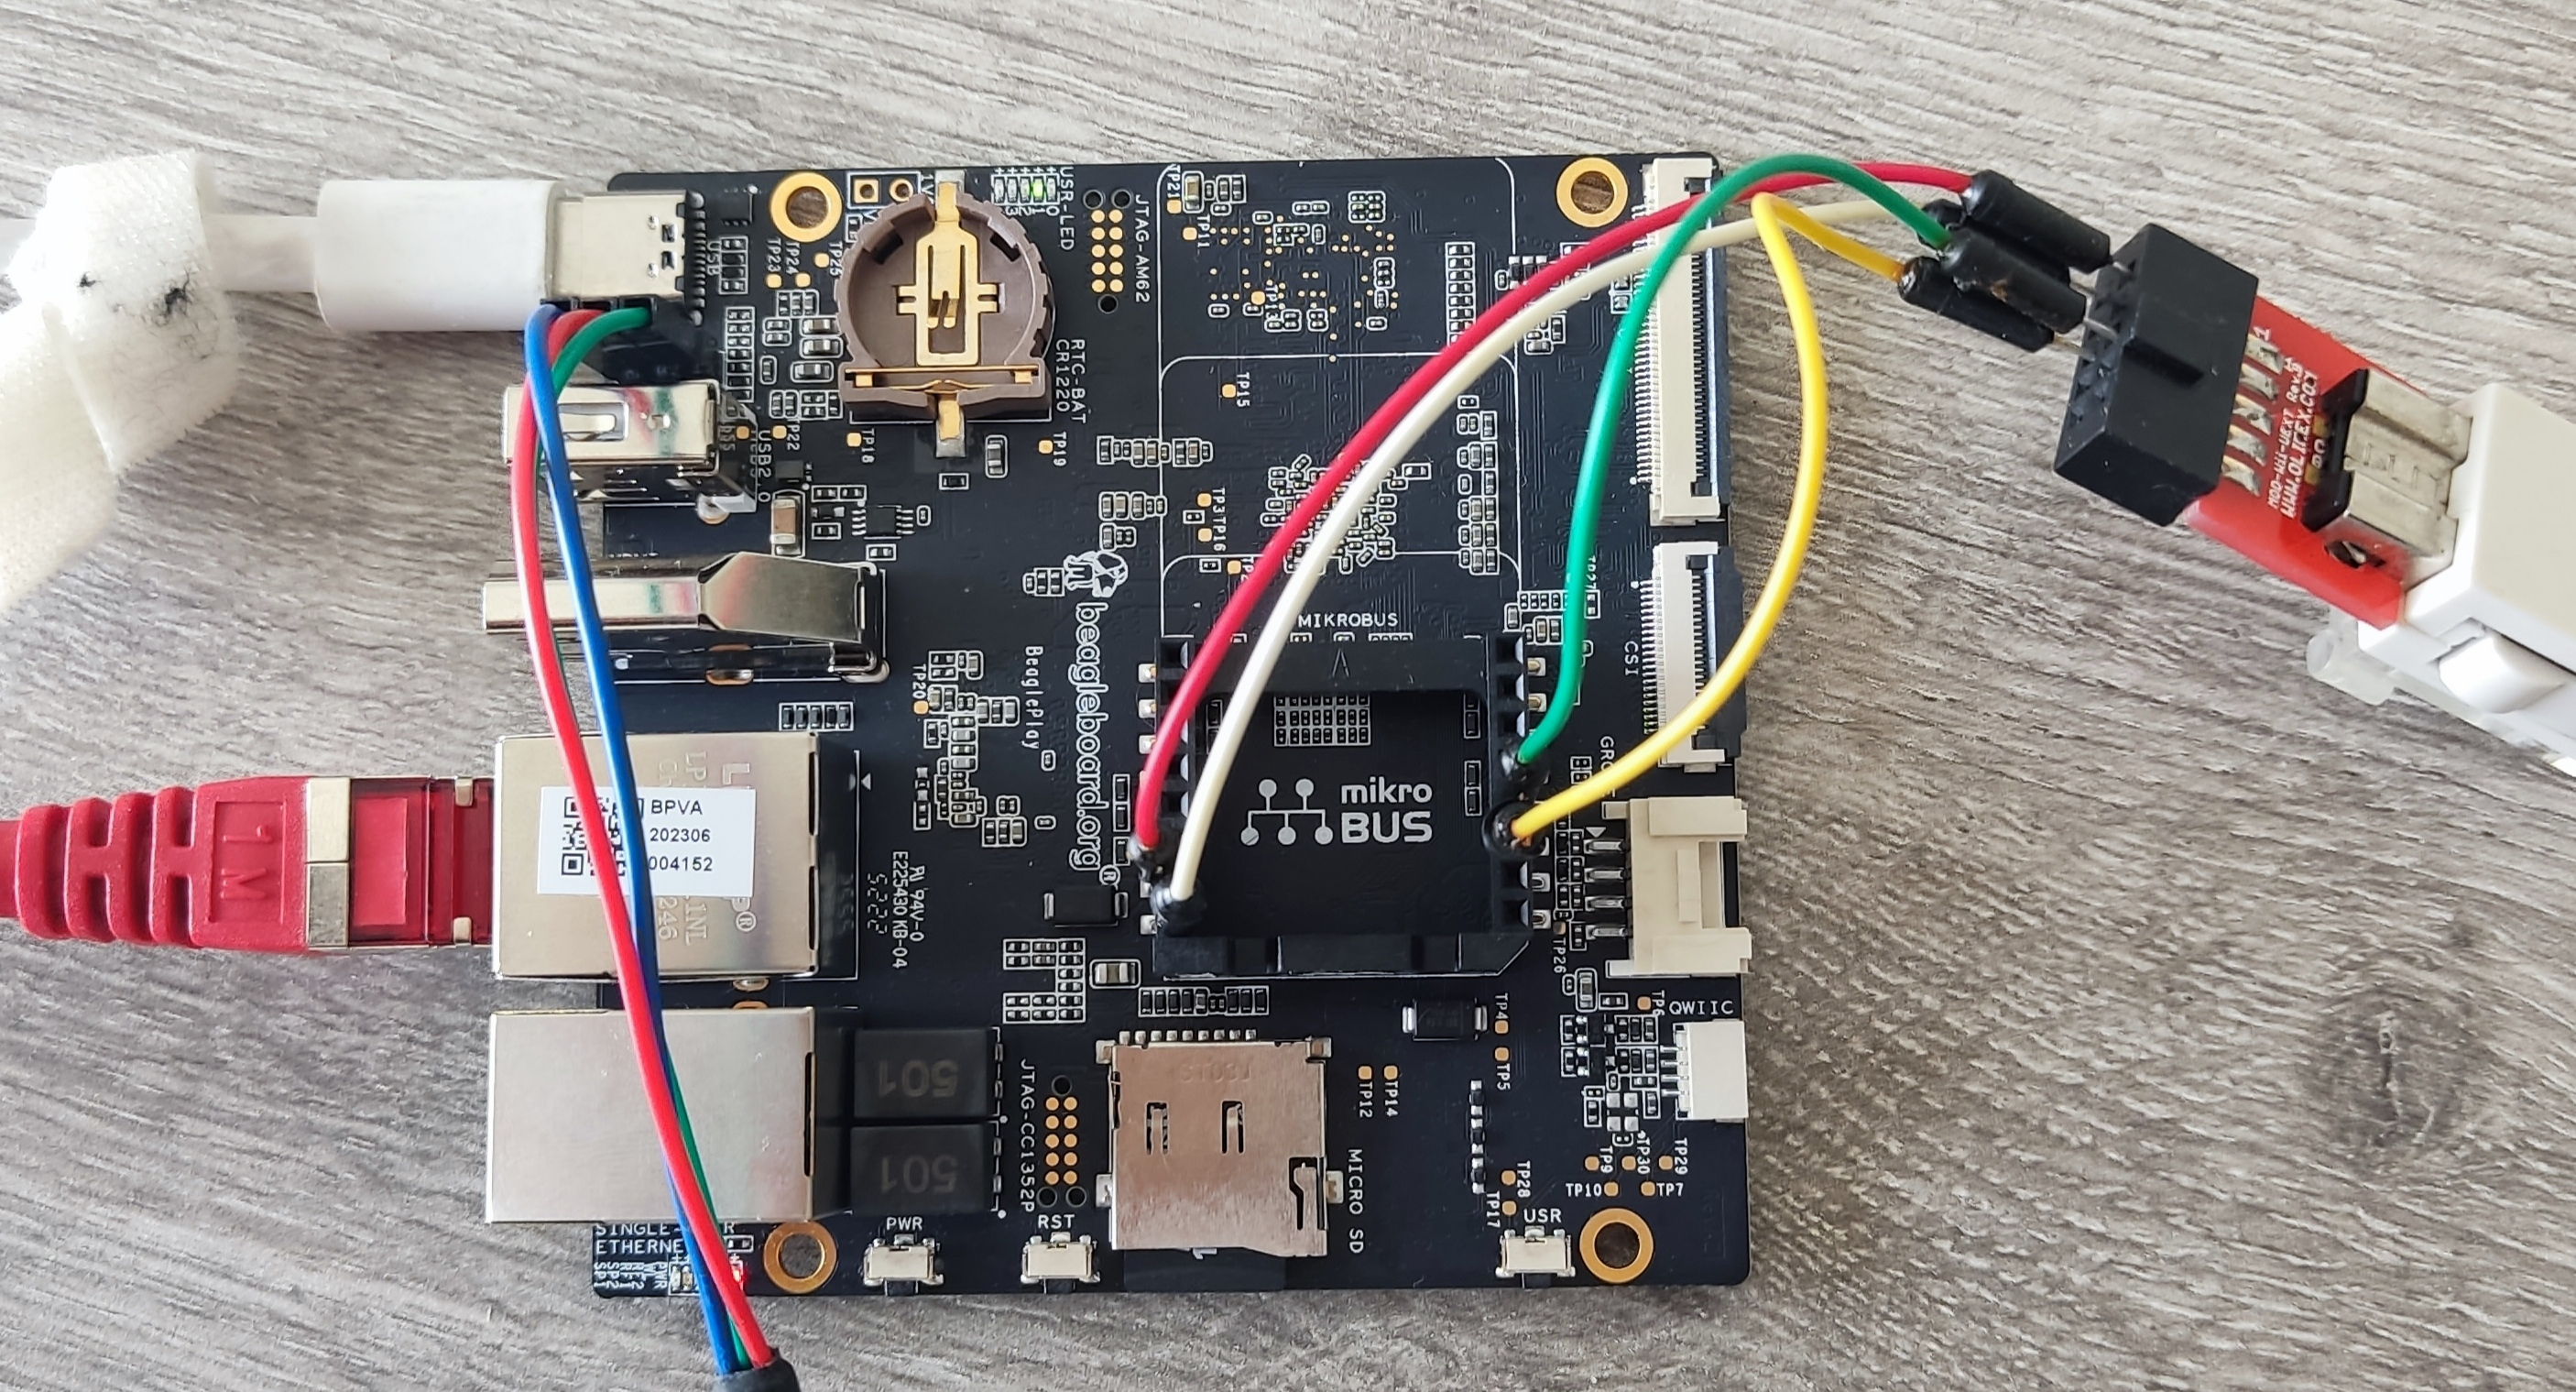
\includegraphics[width=0.7\textwidth]{common/beagleplay-connect-nunchuk.jpg}

In this case, most of the labels on the Mikrobus connector correspond to the
Nunchuk pin names. Just make sure that the PWR Nunchuk pin is connected to the
3.3V mikrobus pin.

If you didn't make any mistakes, your new device should be detected at
address \code{0x52}:

\begin{bashinput}
# i2cdetect -r 3
i2cdetect: WARNING! This program can confuse your I2C bus
Continue? [y/N] y
     0  1  2  3  4  5  6  7  8  9  a  b  c  d  e  f
00:          -- -- -- -- -- -- -- -- -- -- -- -- --
10: -- -- -- -- -- -- -- -- -- -- -- -- -- -- -- --
20: -- -- -- -- -- -- -- -- -- -- -- -- -- -- -- --
30: -- -- -- -- -- -- -- -- -- -- -- -- -- -- -- --
40: -- -- -- -- -- -- -- -- -- -- -- -- -- -- -- --
50: -- -- 52 -- -- -- -- -- -- -- -- -- -- -- -- --
60: -- -- -- -- -- -- -- -- -- -- -- -- -- -- -- --
70: -- -- -- -- -- -- -- --
\end{bashinput}

We will later compile an out-of-tree kernel module to support this device.
